\documentclass[10pt,a4paper]{article}
\usepackage[english]{babel}
\usepackage[utf8]{inputenc}
\usepackage{amsmath}
\usepackage{amsfonts}
\usepackage{amssymb}
\usepackage{graphicx}
\usepackage{float}
\usepackage{url}
\usepackage{caption}

%< > ... dummy content zur Veranschaulichung

\begin{document}
	\part*{Model Documentation of the \\PVTOL with 2 Forces} % MUST - Add Model Name 
	
	%%%%%%%%%%%%%%%%%%%%%% NOMENCLATURE %%%%%%%%%%%%%%%%%%%%%%%%%%%
	
	\section{Nomenclature} % MUST
	\subsection{Nomenclature for Model Equations} % MUST
	
	%variables for model equations
	\begin{tabular}{ll}
		$x$ & horizontal displacement \\
		$y$ & vertical displacement \\
		$\theta$ & roll angle \\
		$F_1$, $F_2$ & Forces on the left and right site of the PVTOL \\
		$g$ & acceleration due to gravity \\
		$l$ & distance between mass center of PVTOL and target point of the forces \\
		$m$ & mass of the PVTOL \\
		$J$ & moment of inertia of the PVTOL		
	\end{tabular}


	\subsection{Graphic of the Structure}	
	\begin{figure}[H]
		\centering
		\captionsetup{justification=centering, margin=1cm}
		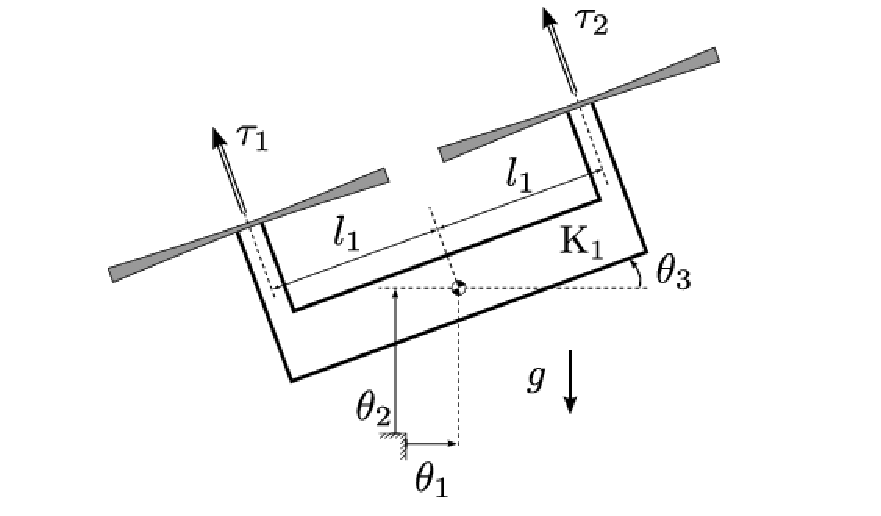
\includegraphics[width=70mm]{pvtol.pdf}
		\caption{Structure of the PVTOL Model. \\ 
		\footnotesize{Source: Knoll, Carsten / \protect\url{https://nbviewer.org/github/cknoll/beispiele/blob/master/senkrechtstarter_pvtol_koordinatentransformation.ipynb}}}
	\end{figure}
	
	%%%%%%%%%%%%%%%%%%%%%% MDOEL EQUATIONS %%%%%%%%%%%%%%%%%%%%%%%%%%%
	
	\section{Model Equations} % MUST
	
	State Vector and Input Vector:
	\begin{align*}
		\underline{x} &= (x_1 \ x_2 \ x_3 \ x_4 \ x_5 \ x_6)^T = (x \ \dot{x} \ y \ \dot{y} \ \theta \ \dot{\theta})^T \\
		\underline{u} &= (u_1 \ u_2)^T = (F_1 \ F_2)^T
	\end{align*}

	\noindent Model Equations:	
	\begin{subequations}
	\begin{align}
		\dot{x}_1 &= x_2 	\\ 
		\dot{x}_2 &= -\frac{\sin(x_5)}{m} (u_1 + u_2)  \\
		\dot{x}_3 &= x_4 \\
		\dot{x}_4 &= \frac{\cos(x_5)}{m} (u_1 + u_2) - g \\
		\dot{x}_5 &= x_6 \\
		\dot{x}_6 &= \frac{l}{J} (u_2 - u_1)
	\end{align}
	\end{subequations}

	%%%%%%%%%%%%%%%%%%%%%% INPUTS| PARAMETERS | OUTPUTS %%%%%%%%%%%%%%%%%%%%%%%%%%%
	\noindent
	Parameters: $m, ~J, ~l, ~g$ % variables with constant, predefined value
	\\
	Outputs:  $x, ~y, ~\theta$% MAY
	
	%%%%%%%%%%%%%%%%%%%%%% ASSUMPTIONS %%%%%%%%%%%%%%%%%%%%%%%%%%%
	
	\subsection{Assumptions} % MAY 
		\begin{enumerate} %possible list type for the Assumptions - mögliche Formatierung für die Annahmen
			\item Forces target the body of the PVTOL in a 90° angle.
		\end{enumerate}
	
	%%%%%%%%%%%%%%%%%%%%%% EXEMPLARY PARAMETER VALUES %%%%%%%%%%%%%%%%%%%%%%%%%%%	
	
	\subsection{Exemplary parameter values}
	\begin{tabular}{cl}
\hline
  Symbol  & Value                                                                                                                                                                                \\
\hline
   $A$    & $\left[\begin{matrix}0.8189 & 0.0863 & 0.09 & 0.0813\\0.2524 & 1.0033 & 0.0313 & 0.2004\\-0.0545 & 0.0102 & 0.7901 & -0.258\\-0.1918 & -0.1034 & 0.1602 & 0.8604\end{matrix}\right]$ \\
   $B$    & $\left[\begin{matrix}0.0045 & 0.0044\\0.1001 & 0.01\\0.0003 & -0.0136\\-0.0051 & 0.0936\end{matrix}\right]$                                                                          \\
 $B_{1}$  & $\left[\begin{matrix}0.0045 & 0.0044\\0.1001 & 0.01\\0.0003 & -0.0136\\-0.0051 & 0.0936\end{matrix}\right]$                                                                          \\
 $C_{1}$  & $\left[\begin{matrix}1.0 & 0 & -1.0 & 0\\0 & 0 & 0 & 0\\0 & 0 & 0 & 0\end{matrix}\right]$                                                                                            \\
   $C$    & $\left[\begin{matrix}1.0 & 0 & 0 & 0\\0 & 0 & 1.0 & 0\end{matrix}\right]$                                                                                                            \\
 $D_{11}$ & $\left[\begin{matrix}0 & 0 & 0\\0 & 0 & 0\\0 & 0 & 0\end{matrix}\right]$                                                                                                             \\
 $D_{12}$ & $\left[\begin{matrix}0 & 0\\1.0 & 0\\0 & 1.0\end{matrix}\right]$                                                                                                                     \\
 $D_{21}$ & $\left[\begin{matrix}0 & 1.0 & 0\\0 & 0 & 1.0\end{matrix}\right]$                                                                                                                    \\
\hline
\end{tabular}

	%%%%%%%%%%%%%%%%%%%%%% DERIVATION & EXPLANATION %%%%%%%%%%%%%%%%%%%%%%%%%%%	
	
	\section{Derivation and Explanation} % SHOULD
	The Lagrangian mechanics was used for the solution.
	%%%%%%%%%%%%%%%%%%%%%% REFERENCES %%%%%%%%%%%%%%%%%%%%%%%%%%%
	
	\begin{thebibliography}{10}		
		\bibitem{KNOLL16}Knoll, Carsten: 
		\textit{Regelungstheoretische Analyse- und Entwurfsansätze für unteraktuierte mechanische Systeme}, p. 169, TU Dresden, 2016.
		\bibitem{KNOLL2}Knoll, Carsten: 
		\textit{Senkrechtstarter in der vertikalen Ebene}, Jupyter Notebook published 2016. \\
		\url{https://nbviewer.org/github/cknoll/beispiele/blob/master/senkrechtstarter_pvtol_koordinatentransformation.ipynb}
	\end{thebibliography}

\end{document}